%%%%%%%%%%%%%%%%%%%%%%%%%%%%%%%%%%%%%%%%%%%%%%%%%%%%%%%%%%%%%%%%%%%%%%
% How to use writeLaTeX: 
%
% You edit the source code here on the left, and the preview on the
% right shows you the result within a few seconds.
%
% Bookmark this page and share the URL with your co-authors. They can
% edit at the same time!
%
% You can upload figures, bibliographies, custom classes and
% styles using the files menu.
%
%%%%%%%%%%%%%%%%%%%%%%%%%%%%%%%%%%%%%%%%%%%%%%%%%%%%%%%%%%%%%%%%%%%%%%

\documentclass[12pt]{article}
\usepackage{adjustbox}
\usepackage{sbc-template}
\usepackage{todonotes}
\usepackage{graphicx,url}
\usepackage{amsmath}
\usepackage{multirow}
\usepackage[utf8]{inputenc}  
\usepackage{babel}
\usepackage[T1]{fontenc}
\usepackage{xspace}
\usepackage{url}
\usepackage{graphicx}
\usepackage{subfig}
%----------
\usepackage{unicode-math}
\usepackage{babel}
\babeltags{br = brazil, en = english}
\usepackage[T1]{fontenc}
\usepackage{xspace}
\usepackage{url}
\usepackage{lipsum} 
%\setmathfont{xits-math.otf}
\usepackage{enumerate}
%\setmathfont[math-style=upright,range={`e,`i}]{xits-math.otf}

%--------------
\sloppy

\title{Calculo Numérico\\Trabalho\_4}


\author{Prof. Dra. Larissa de Freitas \inst{1},\\Guilherme de Souza\inst{1}}

\begin{document} 

\maketitle
\br
%\section{Funções}
%\begin{eqnarray}
%$\lambda x: 5x^{3} - 2x^{2} + 8x - 10$\\
%$\lambda x: 2x^{3} + 5x^{2} + \sin x - 30$\\
%$\lambda x: e^{-x2}\cos x$\\
%    $\lambda x: (x+1)(x-1)(x-3)^{5}\\
%    $\lambda x: (x+2)^{3}\sqrt{x^{2}+1}$
%\end{eqnarray}

\section{Métodos implementados}
\begin{itemize}
  \item Trapezio;
  \item 1/3 de Simpsom;
  \item 3/8 de Simpsom ;
  \item Euler ???;
  \item Runge-Kutta 2a Ordem;
  \item Runge-Kutta 4a Ordem;
  \item Adams;
\end{itemize}

Para execução de tais métodos como, \textbf{Trapezio, 1/3 de Simpsom e 3/8 de Simpsom} foram aplicados na lista de exercícios 11\footnote{Disponivel no AVA:\url{https://ava.ufpel.edu.br/pre/pluginfile.php/318455/mod_resource/content/1/ListaDeExercicios11.pdf}}. Os métodos de \textbf{Euler}, \textbf{Runge-Kutta 2a ordem} e \textbf{4a ordem} utilizou-se a lista de exercícios 12\footnote{Disponivel no AVA:\url{https://ava.ufpel.edu.br/pre/pluginfile.php/320366/mod_resource/content/2/ListaDeExercicios12.pdf}}.


\section{Método do Trapezio}
 O método dos trapazeio é um metodo numerico para aproximação da resolução de um integral definida.
 \[\int_{a}^{b} \! fx \, dx = \]

 Dado que no calculo da integral temos diversos procedimentos para resolução desta integral, seja por substituição, integral por partes, substituição trigonométrica, entre outras. Mas o Método do trapézio por sua vez, nos retorna um valor aproximado independendo do método utilizado.

\begin{figure}[ht]
    \centering
    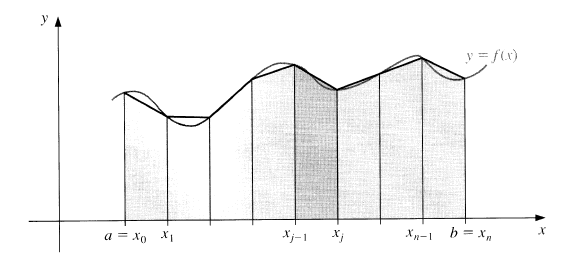
\includegraphics[scale=0.3]{/home/souza/Documents/semestre_2019-2/calculo_numerico/trabalho_4/img/trapezio2.png}
    \caption{Exemplo de de atuação do método dos trapézios}
\end{figure}

Sabemos que a area a limitada pelos limites da integral, como demonstrado na figura 1, o que o método se propoe a realizar a divisão desta area em alguns trapézios ao final realiza sua soma, dessa forma obtendo uma aproximação.


 \[\int_{a}^{b} \! fx \, dx = \sum_{k=1}^{n}Ak \]

%---------------------------------------------------------------------------------------------------
% Resultados 
%---------------------------------------------------------------------------------------------------
\begin{itemize}
    \item \textbf{(B)} Trapezio: 31.365285650063754
\end{itemize}

\begin{table}[ht]
\centering
\begin{tabular}{|lllll|}
-1.08268227 & -0.73575888 & 0.0 & 5.43656366 & 59.11244879
\end{tabular}
    \caption{Função utlizando a regra do trapezio no exercício B da lista 11}
\end{table}


\begin{itemize}
    \item \textbf{(C)} Trapezio: 0.7842407666178157
\end{itemize}

\begin{table}[ht]
\centering
\begin{tabular}{|lllllll|}
  0.5 & 0.97297297 & 0.9 & 0.8 & 0.69230769 & 0.59016393 & 0.25
\end{tabular}
    \caption{Função utlizando a regra do trapezio no exercício C da lista 11}
\end{table}


\begin{itemize}
    \item \textbf{(D)} Trapezio: 0.10486282062502501
\end{itemize}

\begin{table}[ht]
\centering
\begin{tabular}{|lllllll|}
  0.0 & 0.20999043 & 0.69856645 & 1.08060461 & 0.83640026 & -0.53179749 & -1.66458735
\end{tabular}
    \caption{Função utlizando a regra do trapezio no exercício D da lista 11}
\end{table}


\begin{itemize}
    \item \textbf{(E)} Trapezio: -13.575979391799388
\end{itemize}
\begin{table}[ht]
\centering
\begin{tabular}{|lllllllll|}
0.0 & 2.24766465 & 5.42294499 & 6.97416428 & 2.08548731 & -13.92608463 & -39.26843454 & -56.88800791 & -15.25556929
\end{tabular}
    \caption{Função utlizando a regra do trapezio no exercício E da lista 11}
\end{table}


\begin{itemize}
    \item \textbf{(F)} Trapezio: 0.5196110146984233
\end{itemize}
\begin{table}[ht]
\centering
\begin{tabular}{|lllllllll|}
  0.4  & 0.71910112  & 0.64 & 0.56637168 & 0.5 & 0.44137931 & 0.3902439 & 0.34594595 & 0.15384615
\end{tabular}
    \caption{Função utlizando a regra do trapezio no exercício F da lista 11}
\end{table}


\section{Simpsom}

Dando continuidade com métodos de integração, dado a dificuldade de se resolver a integral partindo do principio que muitas vezes se quer há o conhecimento da função, faremos uso do método de Simpsom.

\begin{figure}[!h]
    \centering
    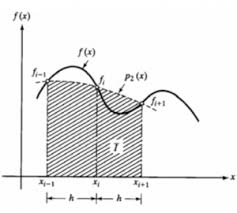
\includegraphics[scale=0.5]{/home/souza/Documents/semestre_2019-2/calculo_numerico/trabalho_4/img/simpson.jpeg}
    \caption{Exemplo de atuação do método de Simpson}
\end{figure}


Dado o exemplo da figura 2, pegamos os dois limites da integral conhecidos e divido em partes suas partes iguais de maneira a encontrar o $h$, como a seguir:

$h=\frac{x_{k+1} - x_{k-1}}{2}$

Dessa forma terei mais pontos sobre o grafico da função, assim interpolando estes pontos, ou seja, procuro qual é o polinomio de menos grau possivel que passe sobre todos, assim calculando a area entre o grafico do polinomio e o intervalo dos eixos do x, esta area é uma aproximação da função f da integral ou seja:


 \[\int_{k-1}^{k+1} \! fx \, dx \approx  \int_{k-1}^{k+1} \! P_{2}x \, dx \]

Pois dessa forma o polinomio é facil de integrar, assim é facil chegar a aproximação da integral. Neste trabalho fizemos uso de dois de seus métodos conhecidos como 1/3 de Simpson, para polinomios de segunda ordem, e 3/8 de Simpson para polinomios de ordem superiores, (a demonstração será ocultada pela vasta demonstração disponvel na internet e pela sua extensa explicação).

Desta forma tais métodos se propoe a serem mais precisos que o métodos do trapézio, geralmente, nem sempre cumprido tal afirmação dada determinada integral e o polnomio.

\subsection{Aplicação de 1/3 de Simpson}
%---------------------------------------------------------------------------------------------------
% Resultados
%---------------------------------------------------------------------------------------------------
\begin{itemize}
    \item \textbf{(B)} 1/3 de Simpsom: 22.231872397453277
\end{itemize}
\begin{table}[ht]
\centering
\begin{tabular}{|lllll|}
 -1.08268227 & -1.47151776 & -0.73575888 & 10.87312731 & 10.87312731
\end{tabular}
    \caption{Função utlizando a regra do trapezio no exercício B da lista 11}
\end{table}


\begin{itemize}
    \item \textbf{(C)} 1/3 de Simpsom: 0.8054718653079309
\end{itemize}
\begin{table}[ht]
\centering
\begin{tabular}{|lllllll|}
     0.5 & 1.94594595 &  0.97297297 & 1.6 & 0.8 & 1.18032787 & 0.29508197
\end{tabular}
    \caption{Função utlizando a regra do trapezio no exercício C da lista 11}
\end{table}


\begin{itemize}
    \item \textbf{(D)} 1/3 de Simpsom: 0.12706697873621364
\end{itemize}
\begin{table}[ht]
\centering
\begin{tabular}{|lllllll|}
     0.0 & 0.41998087 &  0.20999043 & 2.16120922 & 1.08060461 & -1.06359498 & -0.26589874
\end{tabular}
\caption{Função utlizando a regra do trapezio no exercício D da lista 11}
\end{table}


\begin{itemize}
    \item \textbf{(E)} 1/3 de Simpsom: -11.92869601630686
\end{itemize}
\begin{table}[ht]
\centering
\begin{tabular}{|lllllllll|}
    0.0 & 4.49532929  &  2.24766465 & 13.94832857 & 6.97416428 & -27.85216926 & -13.92608463 & -113.77601581  & -28.44400395
\end{tabular}
    \caption{Função utlizando a regra do trapezio no exercício E da lista 11}
\end{table}


\item \textbf(F)} 1/3 de Simpsom: 0.5355245326505693
\end{itemize}
\begin{table}[ht]
\centering
\begin{tabular}{|lllllllll|}
    0.4 & 1.43820225  & 0.71910112 & 1.13274336 & 0.56637168 & 0.88275862 & 0.44137931 & 0.69189189  & 0.17297297
\end{tabular}
    \caption{Função utlizando a regra do trapezio no exercício F da lista 11}
\end{table}


\subsection{Aplicação de 3/8 de Simpsom}


%--------------------------------------------------------------------------------------------------------------------------------
%    Resultados
%--------------------------------------------------------------------------------------------------------------------------------

\item \textbf(B)} 3/8 de Simpsom: 24.405365132780666
\end{itemize}
\begin{table}[ht]
\centering
\begin{tabular}{|lllll|}
    -1.08268227 & -1.10363832 & 0.0 & 8.15484549 & 59.11244879 
\end{tabular}
    \caption{Função utlizando a regra do trapezio no exercício B da lista 11}
\end{table}


\item \textbf(C)} 3/8 de Simpsom: 0.7552413857741727
\end{itemize}
\begin{table}[ht]
\centering
\begin{tabular}{|lllllll|}
    0.5 & 1.45945946 & 1.35 & 1.2 & 0.69230769 & 0.59016393 & 0.25
\end{tabular}
    \caption{Função utlizando a regra do trapezio no exercício C da lista 11}
\end{table}


\item \textbf(D)} 3/8 de Simpsom: 0.2029697091109325
\end{itemize}
\begin{table}[ht]
\centering
\begin{tabular}{|lllllll|}
    0.0 & 0.31498565 & 1.04784968 & 1.62090692 & 0.83640026 & -0.53179749& -1.66458735
\end{tabular}
    \caption{Função utlizando a regra do trapezio no exercício D da lista 11}
\end{table}


\item \textbf(E)} 3/8 de Simpsom: -11.336218635489457
\end{itemize}
\begin{table}[ht]
\centering
\begin{tabular}{|lllllllll|}
    0.0 & 3.37149697 & 8.13441749 & 10.46124643 & 2.08548731 & -13.92608463 & -58.90265182 & -56.88800791 & -15.25556929
\end{tabular}
    \caption{Função utlizando a regra do trapezio no exercício E da lista 11}
\end{table}


\item \textbf(F)} 3/8 de Simpsom: 0.4982574816855577
\end{itemize}
\begin{table}[ht]
\centering
\begin{tabular}{|lllllllll|}
    0.4 & 1.07865169 & 0.96 & 0.84955752 & 0.5 & 0.44137931 & 0.58536585 & 0.34594595 & 0.15384615
\end{tabular}
    \caption{Função utlizando a regra do trapezio no exercício E da lista 11}
\end{table}

\section{Euler}


Como os demais metodos aqui apresentados, o método foca em encontar aproximações de forma a resolver a $fx$. Com tal método é possivel partindo de um ponto conhecido, como, $x_{0}$ $y_{0}$, com isso consigo andar um passo no grafico usando a inclinação da tangente e da secante, ou seja:

$\left \{ \begin{matrix} y' = f(x,y) & \mbox{ }\mbox{ }\\ y(x_{0}) = y_{0} & \mbox{ }\mbox{} \end{matrix} \right.$ 


$h = x_{1} - x_{0}$

$\frac{y_{1} - y_{0}}{h} \approx y'(x_{0})$

$y_{1} - y_{0} \approx hy'(x_{0})$

$y_{1} \approx y_{0} + hy'(x_{0})$

Com isso. apartir do ponto em que está no grafico, é possivel avançar um tamanho $h$ e encontrar o valor $x_{1}$ com isso é possivel encontrar a imagem, $y_{1}$. Ou seja, os novos valores estão bem proximo do grafico da função, dessa forma, basta repetir o metodo mais vezes, de forma a encontrar mais pontos proximos conforme aumenta em um tamanho $h$, a partir do resultado encontrado anteriormente como pode ser visto na figura 3.

\begin{figure}[!h]
    \centering
    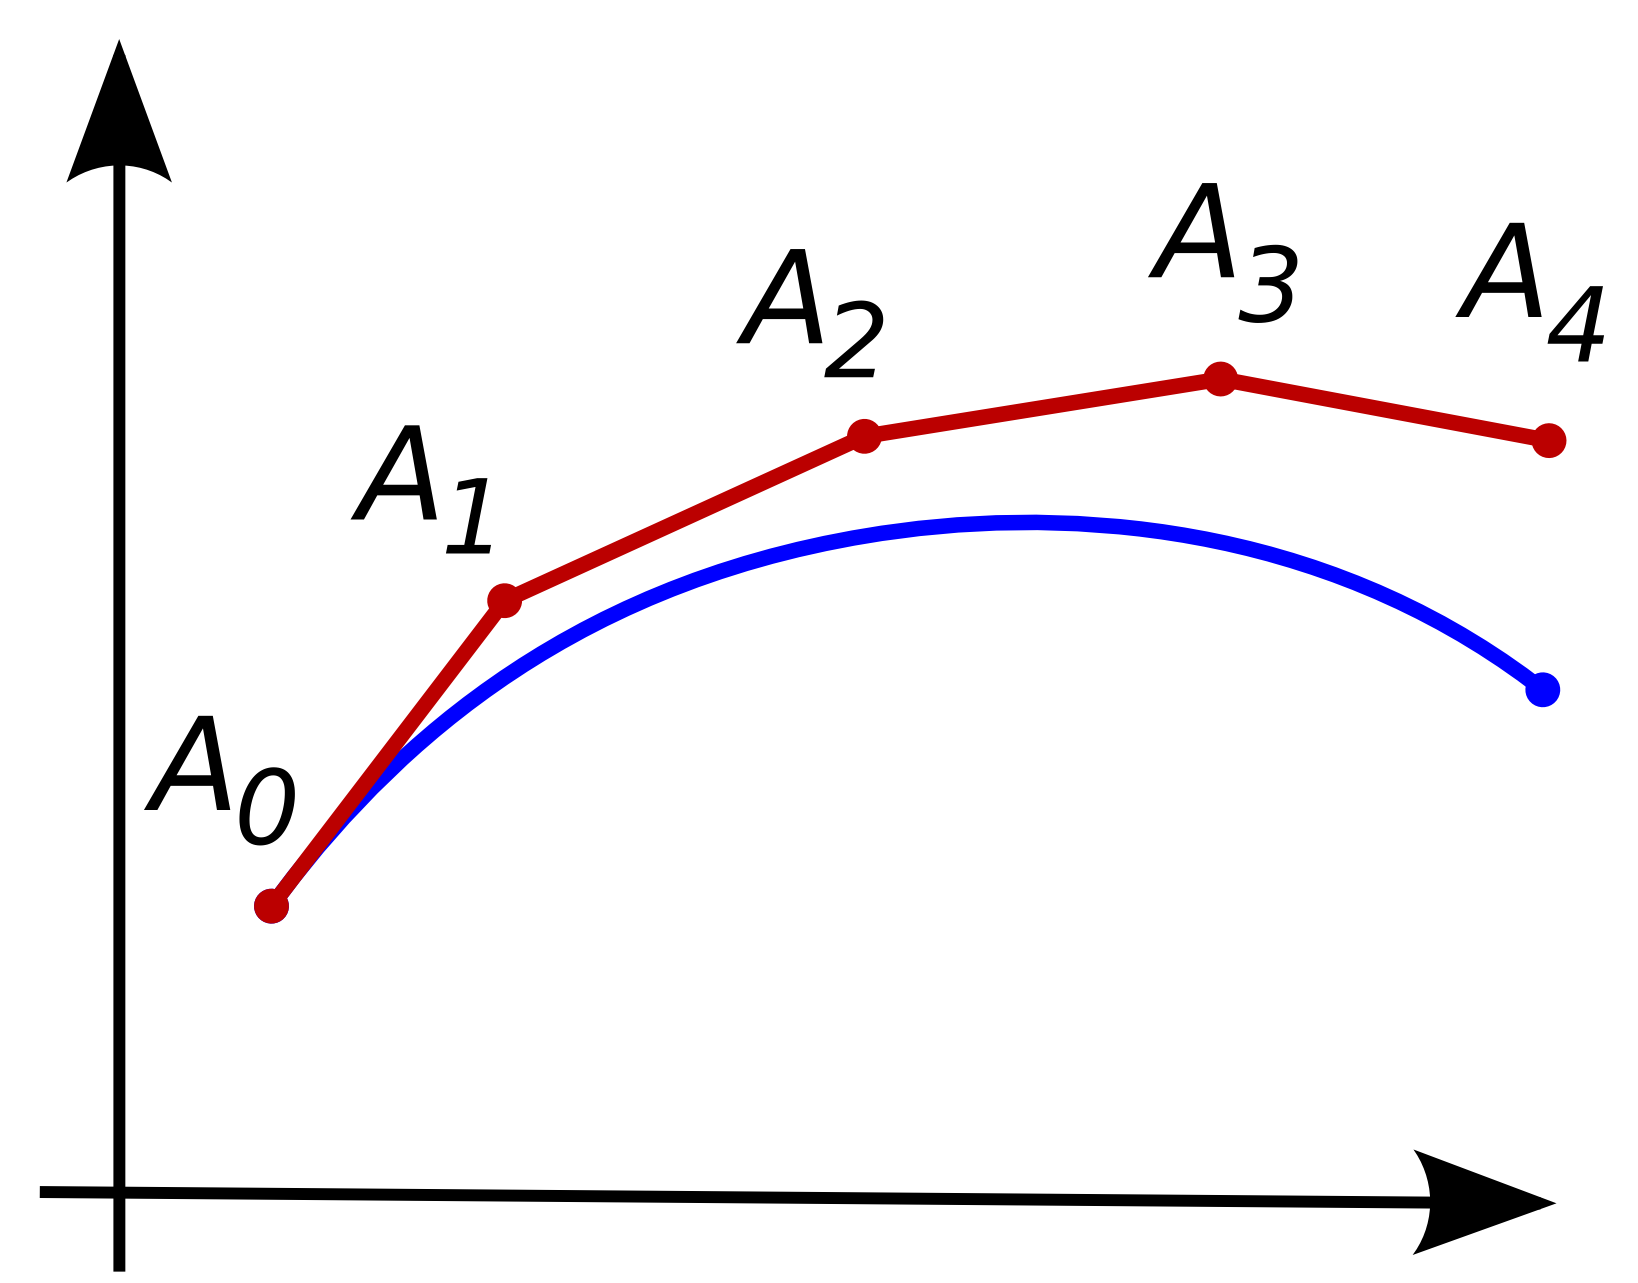
\includegraphics[scale=0.07]{/home/souza/Documents/semestre_2019-2/calculo_numerico/trabalho_4/img/euler.png}
    \caption{Exemplo de atuação do método de Simpson}
\end{figure}

\section{Runge-Kutta 2a ordem}
Dado sua precisão e simplicidade um dos métodos mais utilizados é o método de Runge-kutta. è uma familia de métodos que possuem a precisão dos métodos de Taylor, porém não exige o calculo das derivadas de ordem superior.

A demonstração do método base será ocultada como alguns anteriormente aqui apresentados, dado a sua semelhança na sua primeira ordem ao método de Euler e Taylor de primeira ordem.

\subsection{Runge-Kutta 2a ordem}

Dentre a familia deste método temos o de 2a ordem, que é definido por:

$\omega_{i+1} = \omega_{i} + h(c_{1}k_{1} + c_{2}k_{2})$

com,

$c_{1}$ + $c_{2}$ = 1,

$k_{1}$ = $f(t_{i}$, $\omega_{i}$),

$k_{2}$ = $f(t_{i}$ + $ha_{a}$, $\omega_{i}$ + $h(a_{2}k_{1})$.


Dessa forma podemos determinar $c_{1}$, $c_{2}$ e $a_{2}$, desenvolvendo a função $k_{2}$ pelo polinomio de Taylor, em torno de ($t_{i}, \omega_{i}$) até segunda ordem. Assim acabamos por obter um sistema não linear que possui diversas soluções.

\subsection{Runge-Kutta 4a Ordem}
Através de alguns calculos e algumas mudanças nas variaves tanto da do Runge-Kutta 2a ordem quanto o Runge-Kutta 4-estagios, conseguiremos defirnir um Método de Runge-Kutta 4a ordem.

Através dos calculos chegaremos a um sistema não-linear com solução unica.

\end{document}
